% --- [ Terminology ] ----------------------------------------------------------

\subsection{Terminology}

% ~~~ [ Basic Block ] ~~~~~~~~~~~~~~~~~~~~~~~~~~~~~~~~~~~~~~~~~~~~~~~~~~~~~~~~~~

\subsubsection{Basic Block}

A basic block is a sequence of non-branching instructions terminated by a branching instruction, where incoming branches may only target the first instruction of the basic block and outgoing branches may only leave from the last instruction of the basic block; as illustrated in listing \ref{lst:basic_block}.

\lstinputlisting[language=nasm, style=nasm, label={lst:basic_block}, caption={Examples of basic blocks in x86 assembly.}]{inc/appendices/vocabulary/basic_block.asm}

% ~~~ [ Control Flow Graph ] ~~~~~~~~~~~~~~~~~~~~~~~~~~~~~~~~~~~~~~~~~~~~~~~~~~~

\subsubsection{Control Flow Graph}

A control flow graph $G = (V, E, r)$ is a directed graph rooted at $r$ with vertex set $V$ and edge set $E$, where $r$ denotes the entry point of execution, $v \in V$ denotes a basic block and $(u, v) \in E$ denotes the transfer of control of execution from $u$ to $v$. The corresponding control flow graph of the x86 assembly example in listing \ref{lst:basic_block} is presented in figure \ref{fig:control_flow_graph}.

\begin{figure}[htbp]
	\centering
	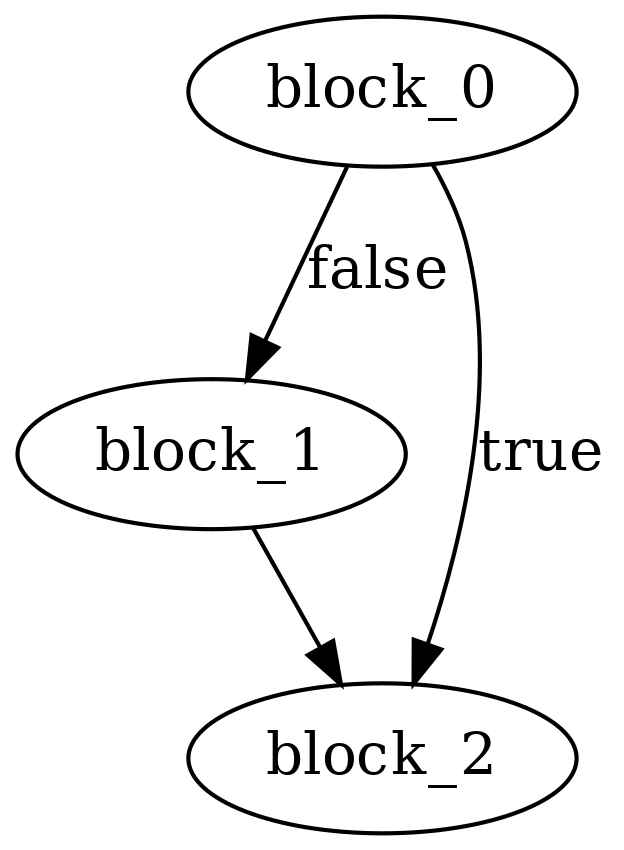
\includegraphics[width=0.2\textwidth]{inc/appendices/vocabulary/control_flow_graph.png}
	\caption{Control flow graph rooted at \texttt{block\_0} corresponding to the x86 assembly example in listing \ref{lst:basic_block}.}
	\label{fig:control_flow_graph}
\end{figure}

% ~~~ [ Interval ] ~~~~~~~~~~~~~~~~~~~~~~~~~~~~~~~~~~~~~~~~~~~~~~~~~~~~~~~~~~~~~

\subsubsection{Interval}

An interval $I(h)$ with header node $h$ is a maximal single-entry subgraph in which $h$ is the only entry node and all cycles contain $h$ \cite{structuring_algorithm_for_decompilation}. The example illustrated in figure \ref{fig:interval} highlights the intervals \textbf{I(B1)}, \textbf{I(B6)}, and \textbf{I(B13)} in a control flow graph.

\begin{figure}[htbp]
	\centering
	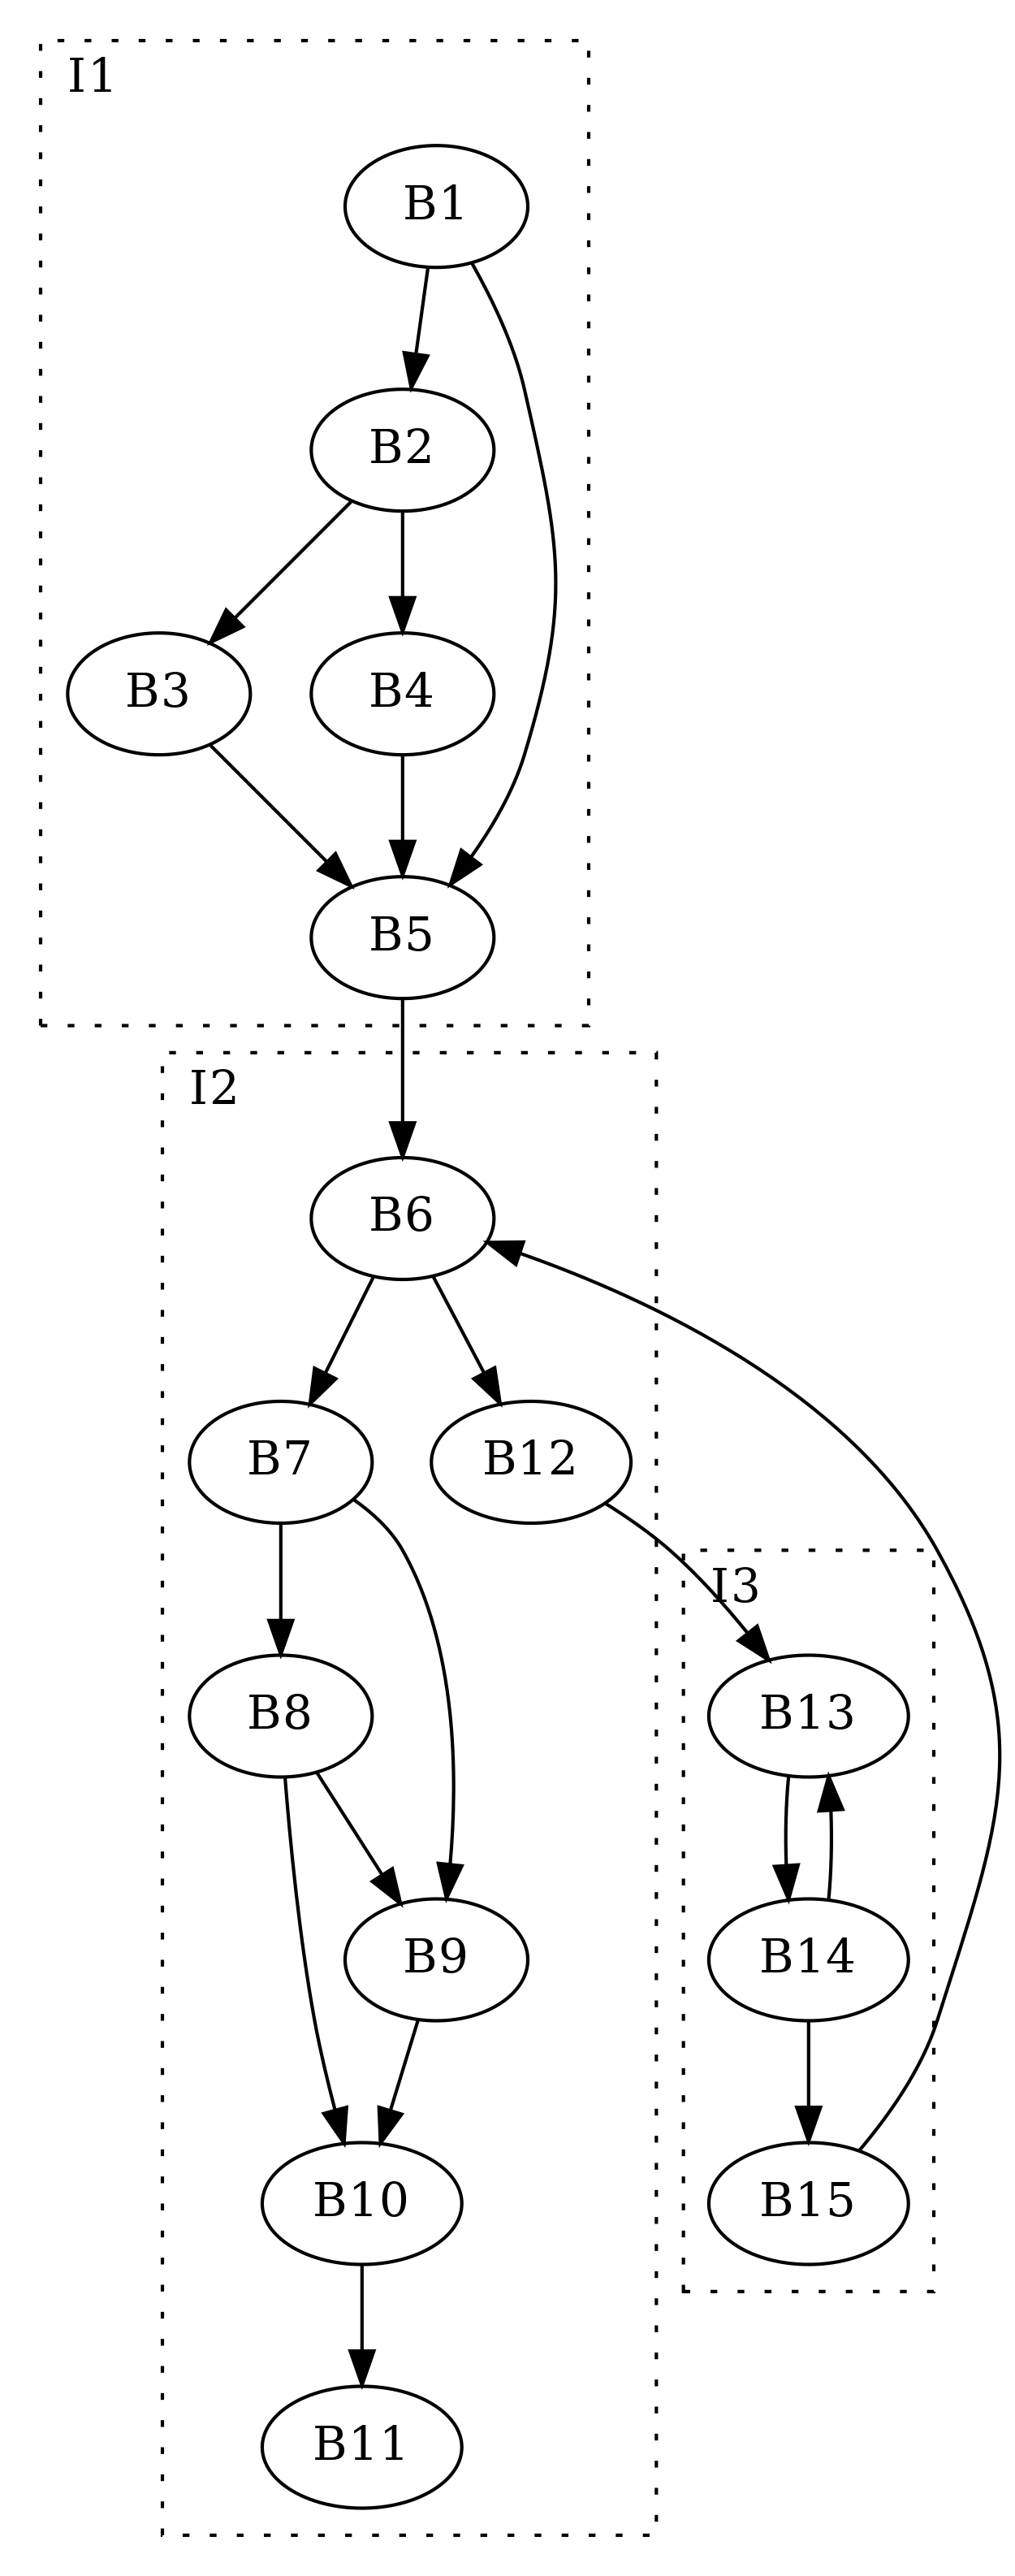
\includegraphics[width=0.3\textwidth]{inc/appendices/vocabulary/interval.png}
	\caption{The intervals \textbf{I1}, \textbf{I2} and \textbf{I3} outlined in a control flow graph; adapted from figure 2 of C. Cifuentes' \textit{Structuring Decompiled Graphs} \cite{structuring_decompiled_graphs}.}
	\label{fig:interval}
\end{figure}

% ~~~ [ Derived Sequence of Graphs G^1...G^n ] ~~~~~~~~~~~~~~~~~~~~~~~~~~~~~~~~~

\subsubsection{Derived Sequence of Graphs}

Given a control flow graph $G$ a derived sequence of graphs, $G^1 \dots G^n$, may be constructed by collapsing intervals. The first order graph $G^1 = G$. The second order graph $G_2$ is obtained by collapsing each interval in $G^1$ into a node. The node of a collapsed interval $I(h)$ has incoming edges from the immediate predecessors of the header node $h$ not part of the interval, and outgoing edges to the immediate successors of the exit nodes of $I(h)$ not part of the interval. The intervals of $G_2$ are collapsed and the process is repeated until $G^n$ is a single node or an irreducible graph.

\todo{TODO: Add illustrations.}

% ~~~ [ Back Edge ] ~~~~~~~~~~~~~~~~~~~~~~~~~~~~~~~~~~~~~~~~~~~~~~~~~~~~~~~~~~~~

\subsubsection{Back Edge}

\todo{TODO: define Back Edge}

% ~~~ [ Reverse Post-order ] ~~~~~~~~~~~~~~~~~~~~~~~~~~~~~~~~~~~~~~~~~~~~~~~~~~~

\subsubsection{Reverse Post-order}

\todo{TODO: define Reverse Post-order}
